\documentclass{report}
\usepackage[T1]{fontenc} % Fontes T1
\usepackage[utf8]{inputenc} % Input UTF8
\usepackage[backend=biber, style=ieee]{biblatex} % para usar bibliografia
\usepackage{csquotes}
\usepackage[portuguese]{babel} %Usar língua portuguesa
\usepackage{blindtext} % Gerar texto automaticamente
\usepackage[printonlyused]{acronym}
\usepackage{hyperref} % para autoref
\usepackage{graphicx}
\usepackage{indentfirst}
\usepackage{lmodern}
\usepackage{epigraph} 
\usepackage[export]{adjustbox}
\usepackage{subcaption}
\usepackage{wrapfig}
\usepackage{multirow}
\usepackage{tabularx}
\usepackage{array}
\usepackage{listings}
\usepackage{xcolor}
\usepackage{geometry} 
\usepackage{titlesec}
\usepackage{amsmath}
\usepackage{booktabs}


\titleformat{\chapter}[display]
  {\normalfont\bfseries}{}{0pt}{\Huge}

\geometry{lmargin=2.5cm,rmargin=2.5cm,bmargin=3cm,tmargin=2.5cm} 

\definecolor{codebackground}{rgb}{0.95,0.95,0.92}
\definecolor{codegreen}{rgb}{0,0.75,0}
\definecolor{codegray}{rgb}{0.5,0.5,0.95}
\definecolor{codepurple}{rgb}{0.58,0,0.82}
\definecolor{codestring}{rgb}{0.82,0.1,0.26}
\definecolor{darkgreen}{rgb}{0,0.35,0}

\lstdefinestyle{CStyle}{
    backgroundcolor=\color{codebackground},
    commentstyle=\color{codegreen},
    keywordstyle=\color{codepurple},
    numberstyle=\tiny\color{codegray},
    stringstyle=\color{codestring},
    basicstyle=\ttfamily\small,
    breakatwhitespace=false,
    breaklines=true,
    captionpos=b,
    keepspaces=true,
    numbers=left,
    numbersep=5pt,
    showspaces=false,
    showstringspaces=false,
    showtabs=false,
    tabsize=4,
    language=C,
    emph={uint8, Image},
    emphstyle=\color{darkgreen}
}

\lstset{style=CStyle}



\begin{document}
%%
% Definições
%
\def\titulo{O TAD image8bit}
\def\data{\today}
\def\autores{José Diogo Cerqueira, Bernardo Marujo}
\def\autorescontactos{(76758) c.jose.diogo@ua.pt, (107322) bernardomarujo@ua.pt}
\def\departamento{Dept. de Eletrónica, Telecomunicações e Informática}
\def\empresa{Universidade de Aveiro}
\def\logotipo{ua.pdf}
%
%%%%%% CAPA %%%%%%
%

%
%
\begin{titlepage}

\begin{center}
%
\vspace*{50mm}
%
{\Huge\textbf{\titulo}}\\
{\Large \departamento\\ \empresa}\\
%
\vspace{10mm}
%
%
{\LARGE \autores\\ \autorescontactos} \\ 
%
\vspace{10mm}
%
\data
%
\vspace{20mm}
%
\begin{figure}[h]
\center
\includegraphics{\logotipo}
\end{figure}
%
\end{center}
%
\end{titlepage}
%%%%%%%%%%%%%%%%%%%%%%%%%%%%%%%%%%%%%%%%%%%%%%%%%%%%%%%%%%%%%%%%%%%%%%%%%%%%%%%%%%%%%%%%%%%%%%
\pagenumbering{roman}


\tableofcontents



\clearpage
\pagenumbering{arabic}


%%%%%%%%%%%%%%%%%%%%%%%%%%%%%%%%%%%%%%%%%%%%%%%%%%%%%%%%%%%%%%%%%%%%%%%%%%%%%%%%%%%%%%%%%%%%%%
\chapter{Introdução}

Neste relatório é apresentado o trabalho prático realizado no âmbito da unidade curricular de Algoritmos e Estruturas de Dados, com dois objetivos principais.
\par
O primeiro é desenvolver desenvolver e testar o TAD (Tipo Abstrato de Dados) \texttt{image8bit}, que permite manipular imagens de 8 bits com com níveis de cinzento, em que cada pixel pode tomar valores de intensidade entre 0 e 255.
\par
O segundo é analisar a complexidade computacional da função \texttt{ImageLocateSubImage} que permite determinar, caso exista, a localização de uma subimagem numa imagem dada, e da função \texttt{ImageBlur} que aplica um filtro a uma imagem e a torna baça.

\hfill

\hfill

\hfill

%%%%%%%%%%%%%%%%%%%%%%%%%%%%%%%%%%%%%%%%%%%%%%%%%%%%%%%%%%%%%%%%%%%%%%%%%%%%%%%%%%%%%%%%%%%%%%
\hspace{-7mm}
{\LARGE\textbf{Estrutura de Dados e Funções do TAD image8bit}}

\section{Estrutura de Dados image8bit}

A estrutura de dados \texttt{image8bit} é composta por um ponteiro para um array de pixeis, um inteiro que representa a largura da imagem, um inteiro que representa a altura da imagem e um inteiro que representa entre que valores vão variar os tons de cinzento dos pixeis, sendo este o valor máximo que um pixel pode assumir, que corresponde à cor branca.
\par
O array de pixeis é um array de unsigned char, em que cada posição do array representa um pixel da imagem, e cada pixel pode tomar valores de intensidade entre 0 e 255 (valor máximo que podemos meter no \textit{maxval}). A posição do pixel (\(x\),\(y\)) no array é dada por \(x\) + \(y\) * (\textit{largura da imagem}).
\par
A estrutura de dados \texttt{image8bit} é definida da seguinte forma:

\begin{lstlisting}[language=C]
struct image {
  int width;
  int height;
  int maxval;   // maximum gray value (pixels with maxval are pure WHITE)
  uint8* pixel; // pixel data (a raster scan)
};
\end{lstlisting}




%%%%%%%%%%%%%%%%%%%%%%%%%%%%%%%%%%%%%%%%%%%%%%%%%%%%%%%%%%%%%%%%%%%%%%%%%%%%%%%%%%%%%%%%%%%%%%
\chapter{Apresentação e Análise da Complexidade Computacional das Funções}

\section{Analise da complexidade da função ImageLocateSubImage}
\subsection{Apresentação}

A função \texttt{ImageLocateSubImage} permite determinar, caso exista, a localização de uma subimagem numa imagem dada.
\par
Para determinar a localização da subimagem, a função percorre a imagem dada e, para cada pixel da imagem, verifica se a subimagem se encontra nessa posição. 
Para verificar se a subimagem se encontra nessa posição, a função percorre a subimagem com a função \texttt{ImageMatchSubImage} e verifica se os pixeis da subimagem são iguais aos pixeis da imagem na posição (x,y) da imagem.
Por este motivo, podemos fazer a análise da complexidade para cada função.
\par
\begingroup
\begin{lstlisting}[language=C]
int ImageLocateSubImage(Image img1, int* px, int* py, Image img2) { ///
  assert (img1 != NULL);
  assert (img2 != NULL);
  assert (px != NULL);
  assert (py != NULL);

  // Search for the subimage in the image
  for (int i = 0; i <= img1->height - img2->height; i++) {
    for (int j = 0; j <= img1->width - img2->width; j++) {
      // If the subimage is found, set the position and end the search
      if (ImageMatchSubImage(img1, j, i, img2)) {
        *px = j;
        *py = i;
        return 1;
      }
    }
  }
  return 0;
}
\end{lstlisting}
    
\begin{lstlisting}[language=C]
int ImageMatchSubImage(Image img1, int x, int y, Image img2) { ///
  assert (img1 != NULL);
  assert (img2 != NULL);
  assert (ImageValidPos(img1, x, y));
  assert (ImageValidRect(img1, x, y, img2->width, img2->height));

  // Compare the pixels of the subimage with the pixels of the image
  for (int i = 0; i < img2->height; i++) {
    for (int j = 0; j < img2->width; j++) {
      ADDS += 1;
      // If the pixels are different, return 0, continuing the search
      if (ImageGetPixel(img1, x + j, y + i) != ImageGetPixel(img2, j, i)) {
        return 0;
      }
    }
  }
  return 1;
}
\end{lstlisting}
\endgroup

\subsection{Análise Formal da Complexidade}

\subsubsection*{ImageMatchSubImage}
A função \texttt{ImageMatchSubImage} tem uma complexidade de \(O(h \cdot w)\), pois itera por cada pixel da subimagem, 
sendo \(h\) e \(w\) a altura e largura da subimagem, respetivamente.
\par

\subsubsection{Complexidade da Função ImageLocateSubImage}

\subsubsection{Melhor Caso}
Se a subimagem for encontrada na primeira posição, a função \texttt{ImageMatchSubImage} será chamada apenas uma vez. 
Portanto, a complexidade no melhor caso é \(O(h \cdot w)\), escalando o tempo de execução, linearmente, com o tamanho da subimagem.

\subsubsection{Pior Caso Num Cenário Real}
No pior caso, os ciclos aninhados iteram sobre todas as posições possíveis dentro da imagem, 
resultando em \((n-h) \cdot (m-w)\) chamadas a \texttt{ImageMatchSubImage}, com \(n\) e \(m\) a altura e largura da imagem, respetivamente. 
Cada chamada a \texttt{ImageMatchSubImage} tem uma complexidade de \(O(h \cdot w)\).
Portanto, a complexidade no pior caso num caso real é \(O((n-h) \cdot (m-w) + h \cdot w)\), escalando o tempo de execução, 
com o tamanho da imagem e da subimagem. Na maioria dos casos existe sempre uma discrepância de aproximadamente 1\% no valor que seria esperado, devido ao facto de existirem pixeis que são iguais aos pixeis que ele encontra na subimagem nas primeiras posições, entrando assim na função \texttt{ImageMatchSubImage} e acionando o contador. Essa diferença de um 1\% são então os pixeis que são iguais aos primeiros pixeis da imagem pequena, parando eventualmente pois só correspondem alguns dos primeiros pixeis.

Para o valor ser exato , teríamos que ter, por exemplo, uma imagem toda preta de base, e uma subimagem, onde o primeiro pixel não é preto. A precisão vai ser de 100\%, pois o contador só começa a contar a partir do momento onde de facto a subimagem aparece.

\vspace{5mm}

\begingroup
\begin{lstlisting}[language=C]
for (i=0; i <= n-h; i++){
    
    for (j=0; j <= m-w; j++){}
}            
for (k=0; k <= h; k++){
            
    for (l=0; l <= w; l++){}
}
\end{lstlisting}
\endgroup

\vspace{5mm}

\begin{equation}
     \sum_{i=0}^{n-h-1}  \hspace{2mm} \sum_{j=0}^{m-w-1} \hspace{2mm} 1 \hspace{2mm} + \hspace{2mm} \sum_{k=0}^{h-1} \hspace{2mm}  \sum_{l=0}^{w-1} \hspace{2mm} 1 \notag
\end{equation}

\newpage

\subsection{Testes Experimentais}


\subsubsection{Exemplo ilustrado para a localização de uma imagem pequena numa grande }

\begin{table}[h]
    \centering
    \begin{tabular}{cccccc}
        \toprule
        \textbf{Case} & \textbf{Position} & \textbf{time} & \textbf{caltime} & \textbf{memops} & \textbf{adds}\\
        \midrule
        Best Case & FOUND (0,0) & 0.000246 & 0.000152 & 131072 & 65536 \\
        Worst Case & FOUND (1344,944) & 0.007787 & 0.004829 & 2675784 & 1337892 \\
        \bottomrule
    \end{tabular}
    \caption{Performance Metrics for LOCATE Operations - Small 256x256 in Large 1600x1200}
\end{table}


\begin{figure}[h]

\begin{subfigure}{0.5\textwidth}
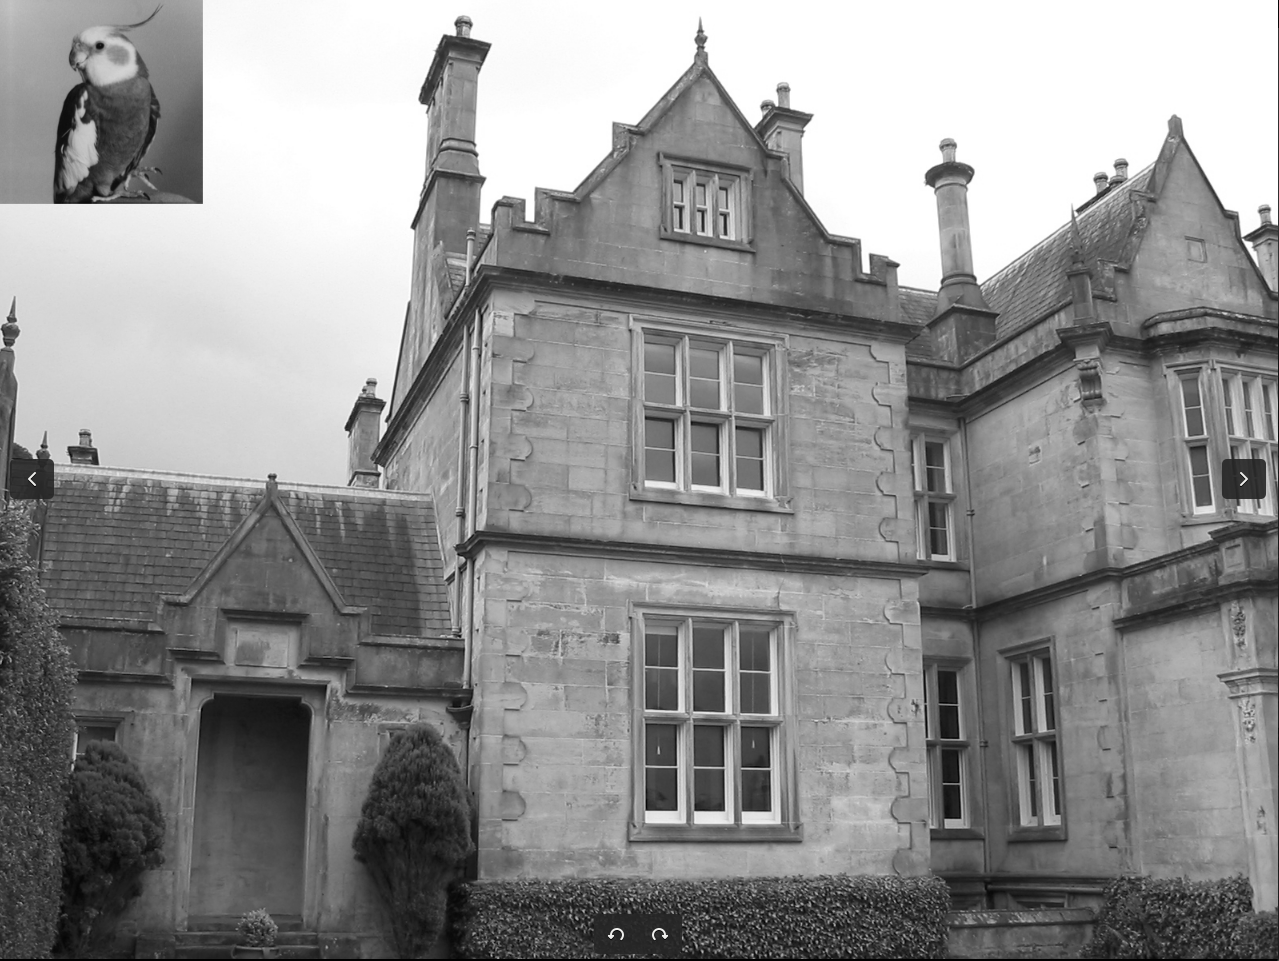
\includegraphics[width=0.9\linewidth, height=6cm]{Screenshot from 2023-11-23 03-27-09.png} 
\caption{Best Case}
\end{subfigure}
\begin{subfigure}{0.5\textwidth}
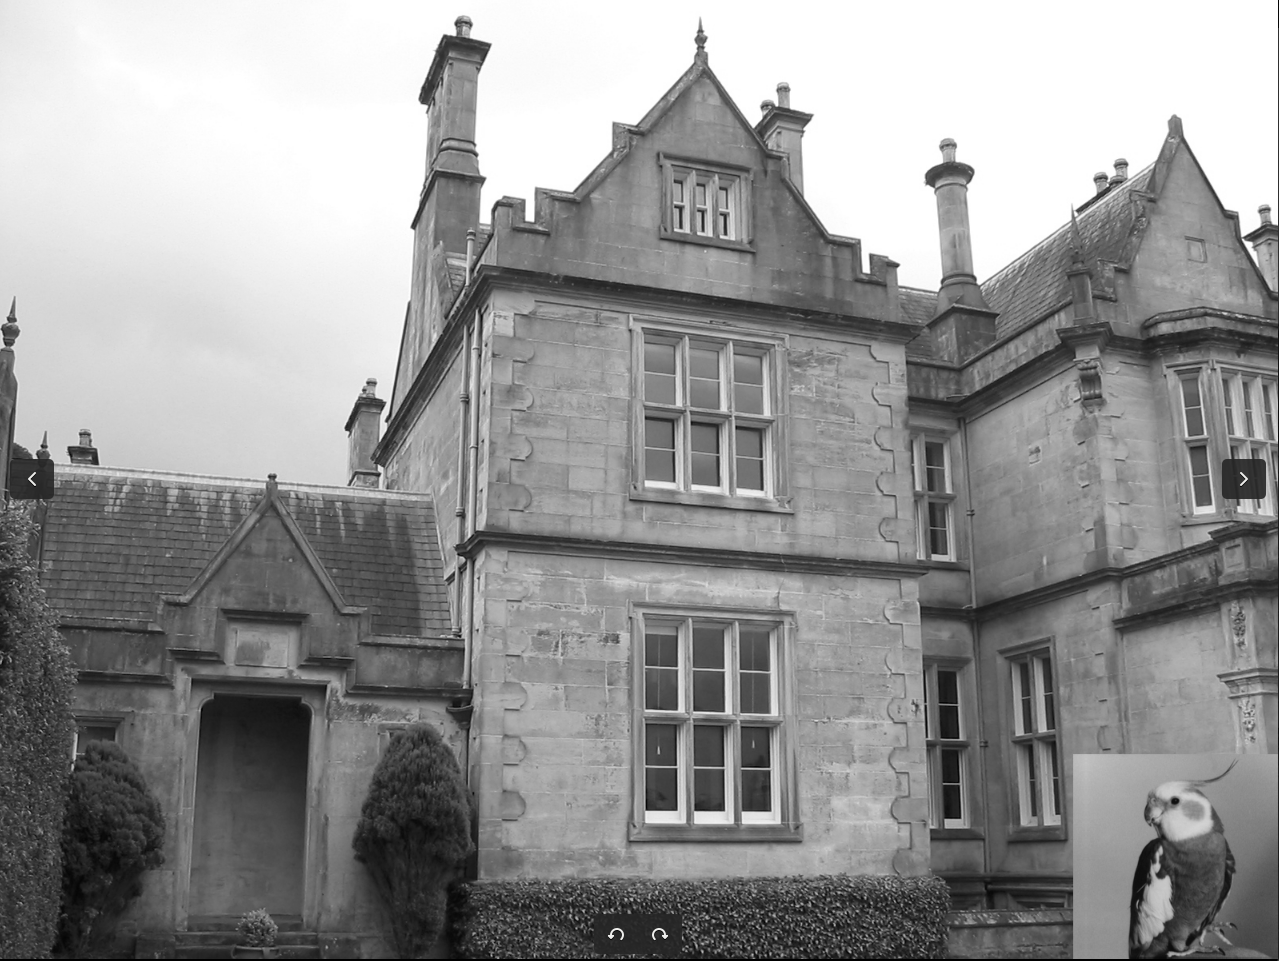
\includegraphics[width=0.9\linewidth, height=6cm]{Screenshot from 2023-11-23 03-26-59.png}
\caption{Worst Case}
\end{subfigure}
\end{figure}

\vspace{-10mm}

\subsubsection{Testes para outros tamanhos}

\subsubsection{Melhor Caso}


\begin{table}[h]
    \centering
    \begin{tabular}{cccccc}
        \toprule
        \textbf{Images Sizes} & \textbf{Position} & \textbf{time} & \textbf{caltime} & \textbf{memops} & \textbf{adds}\\
        \midrule
        Medium 512x512 in Large 1600x1200 & FOUND (0,0) & 0.000919 & 0.000571 & 524288 & 262144 \\
        Large 940x940 in Large 1600x1200 & FOUND (0,0) & 0.003030 & 0.001884 & 1767200 & 883600 \\
        Small 256x256 in Medium 512x512 & FOUND (0,0) & 0.000232 & 0.000145 & 131072 & 65536 \\
        Small 256x256 in Small 300x300 & FOUND (0,0) & 0.000240 & 0.000150 & 131072 & 65536 \\
        \bottomrule
    \end{tabular}
    \caption{Performance Metrics for LOCATE Operations Best Case}
\end{table}

\newpage


\subsubsection{Pior Caso Cenário Real}


\begin{table}[h]
    \centering
    \begin{tabular}{cccccc}
        \toprule
        \textbf{Images Sizes} & \textbf{Position} & \textbf{time} & \textbf{caltime} & \textbf{memops} & \textbf{adds}\\
        \midrule
        Medium 512x512 in Large 1600x1200 & FOUND (1088,688) & 0.005454 & 0.003396 & 2033540 & 1016770 \\
        Large 940x940 in Large 1600x1200 & FOUND (660,260) & 0.004063 & 0.002522 & 2112406 & 1056203 \\
        Small 256x256 in Medium 512x512 & FOUND (256,256) & 0.000635 & 0.000395 & 264036 & 132018 \\
        Small 256x256 in Small 300x300 & FOUND (44,44) & 0.000243 & 0.000151 & 135120 & 67560 \\
        \bottomrule
    \end{tabular}
    \caption{Performance Metrics for LOCATE Operations Worst Case}
\end{table}

\subsection{O Pior Caso}


A complexidade no pior caso é \(O((n-h) \cdot (m-w) \cdot h \cdot w)\), escalando o tempo de execução, quadraticamente, 
com o tamanho da imagem e da subimagem.

Este cenário não é no entanto realista, pois só é possível de ser obtido, se a subimagem fosse repetida várias vezes, apenas com o ultimo pixel diferente, para a imagem não ser igual, exceto na ultima ocorrência da subimagem, onde de facto ela se encontra. Segue-se um exemplo ilustrativo deste caso.


\begin{figure}[h]

\begin{subfigure}{0.5\textwidth}

\includegraphics[width=0.9\linewidth, height=6cm]{Screenshot from 2023-11-24 15-30-46.png}
\caption{Main Image 10x10}
\end{subfigure}
\begin{subfigure}{0.5\textwidth}
\hspace{33mm}

\includegraphics[width=0.15\linewidth, height=1cm]{Screenshot from 2023-11-24 15-33-07.png} 
\caption{Subimage 2x2}
\end{subfigure}
\end{figure}



\begingroup
\begin{lstlisting}[language=C]
for (i=0; i <= n-h; i++){
    
    for (j=0; j <= m-w; j++){
            
    }    for (k=0; k <= h; k++){
            
        }    for (l=0; l <= w; l++){}
}
\end{lstlisting}
\endgroup

\vspace{5mm}

\begin{equation}
     \sum_{i=0}^{n-h-1}  \hspace{2mm} \sum_{j=0}^{m-w-1}  \hspace{2mm} \sum_{k=0}^{h-1} \hspace{2mm}  \sum_{l=0}^{w-1} \hspace{2mm} 1 \notag
\end{equation}


\subsection{Conclusões}

A função ImageLocateSubImage apresenta uma complexidade assintótica significativa, sendo particularmente sensível ao tamanho da imagem e da subimagem. No melhor caso, onde a subimagem é encontrada imediatamente, a complexidade é linear, resultando numa busca eficiente. No entanto, no pior caso (num cenário real), a função escala com as dimensões de ambas as imagens, sendo por isso menos eficiente para, por exemplo, imagens grandes com subimagens pequenas localizadas nas últimas posições da imagem onde está incluída. Por exemplo, para uma imagem pequena (256x256) dentro de uma imagem grande (1600x1200), a quantificação da complexidade do melhor caso é calculada usando apenas as dimensões da imagem pequena, visto esta se encontrar logo no início (  \texttt{$adds = 256\times256 = 65536$}). Já o pior caso (num cenário real) é calculado usando as dimensões de ambas as imagens (\texttt{$adds = (1600-256) \times (1200-256) + 256 \times 256 = 1334272 $}), existindo aquela discrepância nos valores (aproximadamente 1\%).


%%%%%%%%%%%%%%%%%%%%%%%%%%%%%%%%%%%%%%%%%%%%%%%%%%%%%%%%%%%%%%%%
\newpage


\section{Analise da complexidade da função ImageBlur}

\subsection{Apresentação}
Esta função aplica um filtro a uma imagem e a torna baça, tomando como argumentos a imagem e o tamanho do filtro, dado por \(dx\) e \(dy\).
\par
Para calcular o valor de cada pixel da imagem resultante, a função percorre a imagem e, para cada pixel,
calcula a média dos valores dos pixeis da imagem original que se encontram dentro do filtro. Por forma a reduzir a complexidade computacional,
a função \texttt{ImageBlur} utiliza uma matriz auxiliar \texttt{cumSum} que guarda a soma cumulativa dos pixeis anteriores.
\par
Depois de calculada a matriz auxiliar, aplicamos o filtro calculando a média dos valores dos pixeis da imagem original que se encontram dentro do filtro.
\par
A complexidade da função depende apenas do tamanho da imagem, dado que o filtro é calculado percorrendo o array \texttt{cumSum} 
que tem o mesmo tamanho da imagem.
\par
A função \texttt{ImageBlur} é definida da seguinte forma:

\begingroup
\begin{lstlisting}[language=C]
  void ImageBlur(Image img, int dx, int dy) {
    assert(img != NULL);
    assert(dx >= 0);
    assert(dy >= 0);

    int width = img->width;
    int height = img->height;

    // Create an array to store cumulative sums
    double** cumSum = (double**)malloc(height * sizeof(double*));
    for (int i = 0; i < height; i++) {
        cumSum[i] = (double*)malloc(width * sizeof(double));
    }

    // Calculate cumulative sums
    for (int i = 0; i < height; i++) {
        for (int j = 0; j < width; j++) {
            ADDS += 1;

            // Get the value of the current pixel
            cumSum[i][j] = ImageGetPixel(img, j, i);

            // Add the values of the pixels above and to the left
            if (j > 0) {
                cumSum[i][j] += cumSum[i][j - 1];
            }

            if (i > 0) {
                cumSum[i][j] += cumSum[i - 1][j];
            }

            // Subtract the intersection to avoid double addition
            if (i > 0 && j > 0) {
                cumSum[i][j] -= cumSum[i - 1][j - 1];
            }
        }
    }

    // Apply the filter
    for (int i = 0; i < height; i++) {
        for (int j = 0; j < width; j++) {
            ADDS += 1;

            // Calculate the coordinates of the rectangle
            int iMin = (i - dy > 0) ? i - dy : 0;
            int iMax = (i + dy < height - 1) ? i + dy : height - 1;
            int jMin = (j - dx > 0) ? j - dx : 0;
            int jMax = (j + dx < width - 1) ? j + dx : width - 1;

            // Calculate the area of the rectangle
            int area = (iMax - iMin + 1) * (jMax - jMin + 1);

            // Calculate the sum of the pixels inside the rectangle
            double sum = cumSum[iMax][jMax];

            // Subtract the values of the pixels outside the rectangle
            if (iMin > 0) {
                sum -= cumSum[iMin - 1][jMax];
            }
            if (jMin > 0) {
                sum -= cumSum[iMax][jMin - 1];
            }

            // Add the value of the intersection to avoid double subtraction
            if (iMin > 0 && jMin > 0) {
                sum += cumSum[iMin - 1][jMin - 1];
            }

            // Calculate the mean and round it
            uint8 roundedValue = (uint8)(round(sum / area));
            ImageSetPixel(img, j, i, roundedValue);
        }
    }

    // Free the allocated memory
    for (int i = 0; i < height; i++) {
        free(cumSum[i]);
    }
    free(cumSum);
    
}
\end{lstlisting}
\endgroup

\subsection{Análise Formal da Complexidade}

\subsubsection{Inicialização da Matriz de Soma Cumulativa}
A inicialização da matriz de soma cumulativa tem uma complexidade de \(O(n \cdot m)\), pois itera por cada pixel da imagem,
dentro de dois ciclos aninhados, sendo \(n\) e \(m\) a altura e largura da imagem, respetivamente.

\subsubsection{Aplicação do Filtro}
A aplicação do filtro tem uma complexidade de \(O(n \cdot m)\), pois itera por cada posição da imagem, da mesma forma que a inicialização 
da matriz de soma cumulativa. Logo, a complexidade da função \texttt{ImageBlur} é \(O(n \cdot m)\).
\par

\subsubsection{Complexidade global}
Portanto, a complexidade global da função \texttt{ImageBlur} é \(O(n \cdot m)\), considerando que o fator que contribui mais para a complexidade 
é a dimensão da imagem. Isto quer dizer que o desempenho da função \texttt{ImageBlur} é linear em relação à dimensão da imagem.



\subsection{Testes Experimentais}

\begin{table}[h]
    \centering
    \begin{tabular}{ccccc}
        \toprule
        \textbf{BLUR level} & \textbf{time} & \textbf{caltime} & \textbf{memops} & \textbf{adds} \\
        \midrule
        0 & 0.000678 & 0.000421 & 131072 & 131072 \\
        1 & 0.000710 & 0.000441 & 131072 & 131072 \\
        5 & 0.000592 & 0.000368 & 131072 & 131072 \\
        10 & 0.000605 & 0.000376 & 131072 & 131072 \\
        100 & 0.000580 & 0.000360 & 131072 & 131072 \\
        \bottomrule
    \end{tabular}
    \caption*{Performance Metrics for BLUR Operations on \texttt{bird\_256x256.pgm}}
\end{table}


\begin{table}[h]
    \centering
    \begin{tabular}{ccccc}
        \toprule
        \textbf{BLUR level} & \textbf{time} & \textbf{caltime} & \textbf{memops} & \textbf{adds} \\
        \midrule
        0 & 0.002446 & 0.001520 & 524288 & 524288 \\
        1 & 0.002882 & 0.001791 & 524288 & 524288 \\
        5 & 0.002447 & 0.001521 & 524288 & 524288 \\
        10 & 0.002422 & 0.001505 & 524288 & 524288 \\
        100 & 0.002399 & 0.001491 & 524288 & 524288 \\
        \bottomrule
    \end{tabular}
    \caption*{Performance Metrics for BLUR Operations on \texttt{mandrill\_512x512.pgm}}
\end{table}


\begin{table}[h]
    \centering
    \begin{tabular}{ccccc}
        \toprule
        \textbf{BLUR level} & \textbf{time} & \textbf{caltime} & \textbf{memops} & \textbf{adds} \\
        \midrule
        0 & 0.008697 & 0.005390 & 1767200 & 1767200 \\
        1 & 0.009859 & 0.006109 & 1767200 & 1767200 \\
        5 & 0.008381 & 0.005194 & 1767200 & 1767200 \\
        10 & 0.008336 & 0.005165 & 1767200 & 1767200 \\
        100 & 0.008263 & 0.005120 & 1767200 & 1767200 \\
        \bottomrule
    \end{tabular}
    \caption*{Performance Metrics for BLUR Operations on \texttt{einstein\_940x940.pgm}}
\end{table}

\begin{table}[h]
    \centering
    \begin{tabular}{ccccc}
        \toprule
        \textbf{BLUR level} & \textbf{time} & \textbf{caltime} & \textbf{memops} & \textbf{adds} \\
        \midrule
        0 & 0.018296 & 0.011327 & 3840000 & 3840000 \\
        1 & 0.022019 & 0.013632 & 3840000 & 3840000 \\
        5 & 0.019351 & 0.011980 & 3840000 & 3840000 \\
        10 & 0.018723 & 0.011591 & 3840000 & 3840000 \\
        100 & 0.019255 & 0.011921 & 3840000 & 3840000 \\
        \bottomrule
    \end{tabular}
    \caption*{Performance Metrics for BLUR Operations on \texttt{ireland\_03\_1600x1200.pgm}}
\end{table}

\newpage

\subsection{Conclusões}

Conseguimos confirmar que se verifica experimentalmente, aquilo que se esperava pela análise formal da complexidade. 
A quantificação da complexidade, dada por \(adds\), escala linearmente com o tamanho da imagem e 
conseguimos determinar \(adds\) pela multiplicação de \(image\char`_height\) por \(image\char`_length\). 
Por exemplo para a imagem \texttt{einstein\char`_940x940.pgm} temos \texttt{$adds = 940\times940 = 1767200$}.
\par
Verifica-se também que a intensidade de \(blur\), não impacta em nada o desempenho da função, sendo igual o número de \(memops\) e \(adds\) 
para todos os níveis de intensidade.


\section{Análise da complexidade da função ImageWorstBlur}

\subsection{Apresentação}
Para aprensentar uma função menos eficiente, criamos a função \texttt{ImageWorstBlur}, onde o filtro é calculado sem utilizar a matriz auxiliar,
calculando a média dos valores do filtro a cada iteração, percorrendo a imagem original e o filtro.
\par
A função \texttt{ImageWorstBlur} é definida da seguinte forma:

\begingroup
\begin{lstlisting}[language=C]
void WorseImageBlur(Image img, int dx, int dy) {
  assert(img != NULL);
  assert(dx >= 0);
  assert(dy >= 0);
  
  // Create a copy of the image
  int pixelsize = img->width * img->height;
  Image img_copy = ImageCreate(img->width, img->height, img->maxval);
  img_copy->pixel = (uint8*)malloc(pixelsize * sizeof(uint8));
  memcpy(img_copy->pixel, img->pixel, pixelsize * sizeof(uint8));
  
  // Apply the filter
  for (int i = 0; i < img->height; i++) {
      for (int j = 0; j < img->width; j++) {
          double sum = 0.0;
          int count = 0;
          // Calculate the coordinates of the rectangle
          for (int k = i - dy; k <= i + dy; k++) {
              for (int l = j - dx; l <= j + dx; l++) {
                  ADDS += 1;
                  // Check if the pixel is inside the image
                  if (ImageValidPos(img, l, k)) {
                    // Add the value of the pixel to the sum
                    sum += ImageGetPixel(img_copy, l, k);
                    count++;
                  }
              }
          }

          // Calculate the mean and round it
          uint8 roundedValue = (uint8)(round(sum / count));
          ImageSetPixel(img, j, i, roundedValue);
      }
  }
  // Free the allocated memory
  free(img_copy->pixel);
  free(img_copy);
}
\end{lstlisting}
\endgroup

\subsection{Análise Formal da Complexidade}

\subsubsection{Cópia da Imagem}
A cópia da imagem tem uma complexidade de \(O(n \cdot m)\), onde \(n\) e \(m\) são a altura e largura da imagem, respetivamente.

\subsubsection{Aplicação do Filtro}
A aplicação do filtro tem uma complexidade de \(O(n \cdot m \cdot (2 \cdot dy + 1) \cdot (2 \cdot dx + 1))\), 
onde \(n\) e \(m\) são a altura e largura da imagem, respetivamente, 
\(dx\) e \(dy\) são a largura e altura do filtro, respetivamente.
\par
O loop externo itera sobre a altura da imagem (\(n\)) e o loop interno itera sobre a largura da imagem (\(m\)).
\par
Para cada pixel, há um loop adicional que itera sobre uma região retangular de tamanho \((2 \cdot dy + 1) \cdot (2 \cdot dx + 1)\).
\par
Portanto, a complexidade geral da função \texttt{WorseImageBlur} é \(O(n \cdot m \cdot (2 \cdot dy + 1) \cdot (2 \cdot dx + 1))\), 
qe aumenta quadraticamente com o tamanho da imagem e do filtro.


\subsubsection{Complexidade global}
Em suma, a complexidade global da função \texttt{WorseImageBlur} é \(O(n \cdot m \cdot (2 \cdot dy + 1) \cdot (2 \cdot dx + 1))\). 
A complexidade desta função é significativamente maior do que a da função original \texttt{ImageBlur},
especialmente devido aos loops aninhados para a cópia e à região considerada para a aplicação do filtro.


\subsection{Testes Experimentais}

\begin{table}[h]
    \centering
    \begin{tabular}{ccccc}
        \toprule
        \textbf{BLUR level} & \textbf{time} & \textbf{caltime} & \textbf{memops} & \textbf{adds} \\
        \midrule
        0 & 0.000442 & 0.000273 & 131072 & 65536 \\
        1 & 0.001798 & 0.001111 & 652292 & 589824 \\
        5 & 0.017095 & 0.010563 & 7827332 & 7929856 \\
        10 & 0.065231 & 0.040305 & 27796292 & 28901376 \\
        20 & 0.231442 & 0.143006 & 101591312 & 110166016 \\
        \bottomrule
    \end{tabular}
    \caption*{Performance Metrics for WORSE BLUR Operations on \texttt{bird\_256x256.pgm}}
\end{table}

\newpage


\begin{table}[h]
    \centering
    \begin{tabular}{ccccc}
        \toprule
        \textbf{BLUR level} & \textbf{time} & \textbf{caltime} & \textbf{memops} & \textbf{adds} \\
        \midrule
        0 & 0.001611 & 0.001002 & 524288 & 262144 \\
        1 & 0.007232 & 0.004499 & 2615300 & 2359296 \\
        5 & 0.068682 & 0.042722 & 31644548 & 31719424 \\
        10 & 0.263131 & 0.163674 & 113514308 & 115605504 \\
        20 & 0.932412 & 0.579981 & 423469328 & 440664064 \\
        \bottomrule
    \end{tabular}
    \caption*{Performance Metrics for WORSE BLUR Operations on \texttt{mandrill\_512x512.pgm}}
\end{table}



\begin{table}[h]
    \centering
    \begin{tabular}{ccccc}
        \toprule
        \textbf{BLUR level} & \textbf{time} & \textbf{caltime} & \textbf{memops} & \textbf{adds} \\
        \midrule
        0 & 0.005478 & 0.003387 & 1767200 & 883600 \\
        1 & 0.024206 & 0.014966 & 8824724 & 7952400 \\
        5 & 0.231706 & 0.143263 & 107179700 & 106915600 \\
        10 & 0.885484 & 0.547493 & 386220500 & 389667600 \\
        20 & 3.153342 & 1.949705 & 1454018000 & 1485331600 \\
        \bottomrule
    \end{tabular}
    \caption*{Performance Metrics for WORSE BLUR Operations on \texttt{einstein\_940x940.pgm}}
\end{table}

\begin{table}[h]
    \centering
    \begin{tabular}{ccccc}
        \toprule
        \textbf{BLUR level} & \textbf{time} & \textbf{caltime} & \textbf{memops} & \textbf{adds} \\
        \midrule
        0 & 0.011627 & 0.007232 & 3840000 & 1920000 \\
        1 & 0.051778 & 0.032206 & 19183204 & 17280000 \\
        5 & 0.504233 & 0.313629 & 233316900 & 232320000 \\
        10 & 1.925805 & 1.197837 & 842184100 & 846720000 \\
        20 & 6.851739 & 4.261733 & 3181400400 & 3227520000 \\
        \bottomrule
    \end{tabular}
    \caption*{Performance Metrics for WORSE BLUR Operations on \texttt{ireland\_03\_1600x1200.pgm}}
\end{table}


\subsection{Conclusões}

A função WorseImageBlur apresenta uma complexidade quadrática \(O(n \cdot m \cdot (2 \cdot dy + 1) \cdot (2 \cdot dx + 1))\) devido à introdução de uma cópia da imagem e a uma região expandida para aplicação do filtro. Esta contrasta com a versão original ImageBlur, que possui complexidade linear em relação ao tamanho da imagem. Por exemplo para a imagem \texttt{einstein\char`_940x940.pgm} aplicando um filtro (20,20) temos \texttt{$adds = 940\times940\times(2\times20+1)\times(2\times20+1) = 1485331600$}.
\par A eficiência computacional da função é fortemente influenciada pelas dimensões da imagem e do filtro, destacando a importância da otimização algorítmica em operações de processamento de imagem, o que reforça a relevância de abordagens mais simples para alcançar desempenho mais eficaz em cenários intensivos em processamento de imagem.
%%%%%%%%%%%%%%%%%%%%%%%%%%%%%%%%%%%%%%%%%%%%%%%%%%%%%%%%%%%%%%%%%%%%%%%%%%%%%%%%%%%%%%%%%%%%%%


\end{document}
